\section{Results} \label{sec:results}
With the code developed, several tests have been performed to assess the viability of the proposed solution. Even if the underlying idea of fitting functions using neural networks seems interesting, evidence shows non-promising results.

The main issue can be related to the dataset generation and model training. Considering a case with 4 turrets, the goal is to fit a function $\vett f:\ \mathcal X \subset \mathbb R^{11} \rightarrow \mathbb R^{3}$; to have a good and reliable approximation, the whole space $\mathcal X$ should be \textit{sufficiently visited} from a numerical standpoint.

Working from my laptop, even tough minimization problems can be solved as fast as $1ms$, generating $1\,000\,000$ data points requires almost 30 minutes; furthermore with such generated data, each deep-learning model requires about 1 hour to train over 100 epochs. \\
With such amount of data, still the process of training the neural network fails to achieve satisfactory results, probably due to the lack of data that enables a proper function fitting.

\vspace{3mm}
The potentiality of the tool is well expressed when controlling the voltage to be applied to the BLDC motor; such problem requires the fitting of a function $f:\ \mathcal X \subset \mathbb R^{3} \rightarrow \mathbb R$ with a domain of smaller size for which the computation of a sufficiently large data-set is viable.

As exposed in Fig. \ref{fig:motorNN}, models with different configurations of hidden layers are able to reach and correctly track the reference trajectory asked the system.
\begin{figure}[bt]
    \centering
    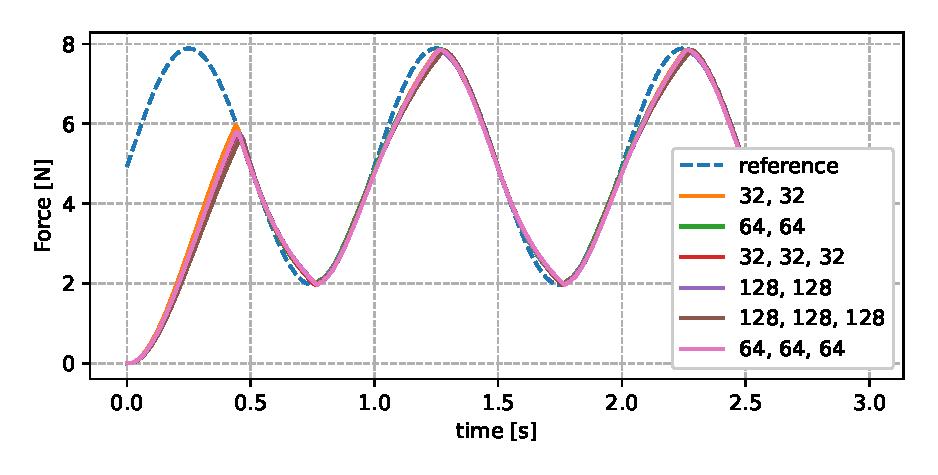
\includegraphics[width=\linewidth]{Images/motorNN.eps}
    \caption{response of different controllers to a sinusoidal input. For each model the number of perceptron in each hidden layer is reported, e.g "32, 32" means \textit{2 hidden layers with 32 perceptrons each}.}
    \label{fig:motorNN}
\end{figure}

\vspace{3mm}

Using one of the above models and solving the allocation problem (\ref{eq:allocproblem}) at each control step shows the desirable behavior in a trajectory-tracking scenario. Considering the 8-shaped trajectory described by
\[ \vett p =
\begin{pmatrix}
    \rho_{x} \cos(c_{1} t) \\ \rho_{y} \sin(c_{2}t) \\ 0
\end{pmatrix}
\]
then Fig. \ref{fig:path} shows the path followed by the ROSPO considering simulation parameters in Table \ref{tab:simdata} and having chosen the feedback matrix $\matt K$ for which the eigenvalues of the close-loop matrix $\matt A - \matt{KB}$ are $(-3,-3,-3)$. Figure \ref{fig:error} reports a more detailed look at the time behavior of the different $x, y$ and $\psi$ component of the state. Finally, Fig. \ref{fig:force} shows how the allocator responds to the commanded virtual input.

\begin{table}[bt]
    \centering
    \caption{coefficients used in the ROSPO simulation.}
    \label{tab:simdata}
    \begin{tabular}{c c}
        parameter & value \\ \hline \hline
        $\rho_{x}$ & $1m$ \\
        $\rho_{y}$ & $0.6m$ \\
        $c_{1}$ & $0.4$ \\
        $c_{2}$ & $0.8$ \\
        $\gamma_{P}$ & $2.5$ \\
        $k_{p}$ & $1.2$ \\
        $k_{d}$ & $1.4$ \\
        $k_{p, \psi}$ & $3.2$ \\
        $k_{d, \psi}$ & $6.35$ \\
        $\gamma_{4}$ & $0.44$ \\
        $\gamma_{5}$ & $1$ \\
        $m$ & $6kg$ \\
        $J$ & $6.1kg\cdot m^{2}$
    \end{tabular}
\end{table}


\begin{figure}[bt]
    \centering
    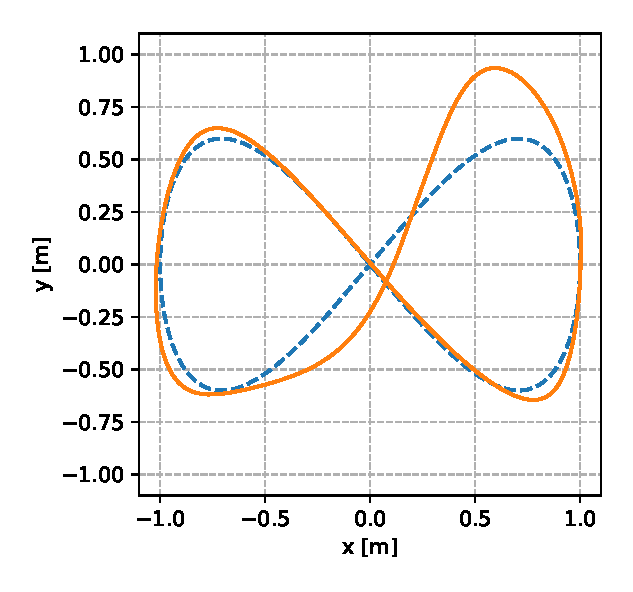
\includegraphics[width=5cm]{Images/path.eps}
    \caption{path followed by the ROSPO while prompted to follow the 8-shaped trajectory.}
    \label{fig:path}
\end{figure}
\begin{figure}[bt]
    \centering
    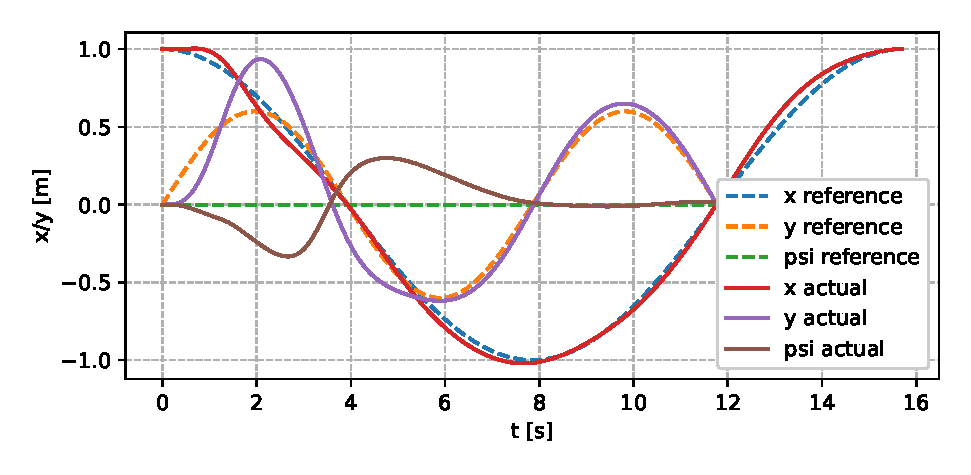
\includegraphics[width=\linewidth]{Images/delta.eps}
    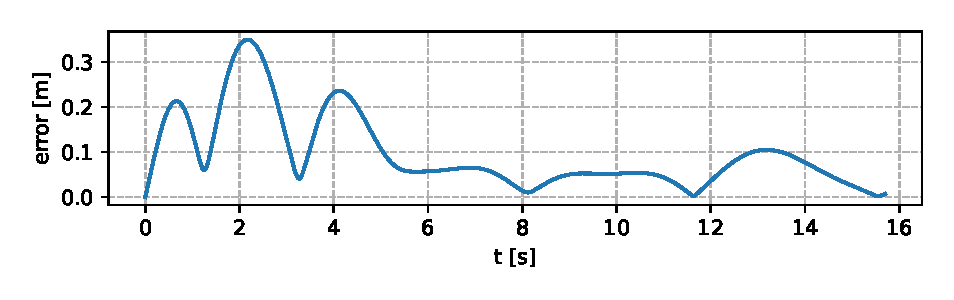
\includegraphics[width=\linewidth]{Images/error.eps}
    \caption{desired and actual position and orientation of the ROSPO during the simulation.}
    \label{fig:error}
\end{figure}
\begin{figure}[bt]
    \centering
    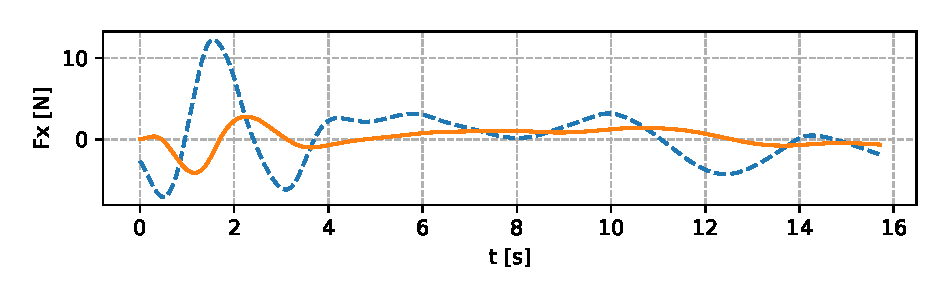
\includegraphics[width=\linewidth]{Images/force-1.eps}
    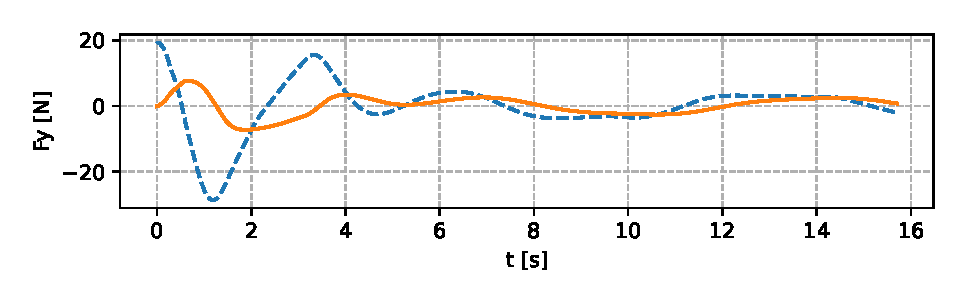
\includegraphics[width=\linewidth]{Images/force-2.eps}
    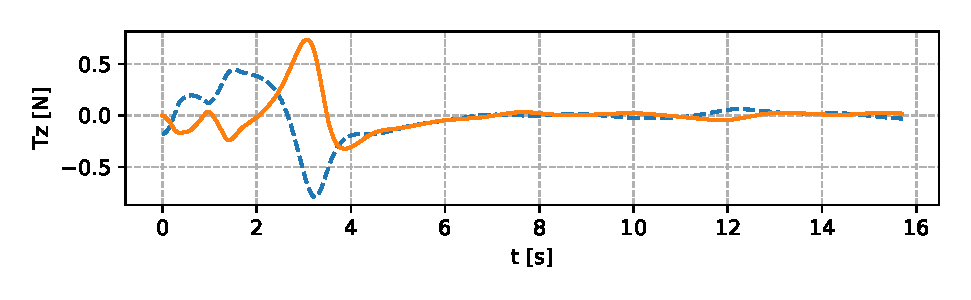
\includegraphics[width=\linewidth]{Images/force-3.eps}
    \caption{commanded virtual input and actual force exherted by the system as function of time in the cardinal directions and resulting torque.}
    \label{fig:force}
\end{figure}

At the beginning, due to a standstill initial condition, the controller isn't capable of following the requested trajectory, and goes into severe errors while following the path; toward the end instead the system converges to the desired trajectory as expected.
